

\chapter{Correlated and Uncorrelated Systematic Uncertainties}

%\section{b-tagging Systematics}

\section{Trigger and Lepton Selection Efficiency}

To calculate the lepton efficiency we use the tag and probe method. This method is a way to use a data sample of pure leptons from Z boson decays to find efficiencies.  We require our events to contain a minimum of two leptons from a Z decay as well as a minimum of one jet.  This matches the event topology that we use in the analysis. The requirements for tag and probe events are shown in Table~\ref{tab:tagandprobe_requirements}. After measuring efficiency in data by applying the same method to measure simulation efficiency, we are able to calculate the scale factors for data to simulation. The complete efficiency measurement can be split into five relative measurements: tracking efficiency, reconstruction efficiency, identification efficiency, isolation efficiency , and the total trigger efficiency.  This is expressed in equation (\ref{eq:efficiency_eq}).
\begin{equation}
\epsilon_{lepton} = \epsilon_{tracking} \times \epsilon_{RECO/tracking} \times \epsilon_{ID/RECO} \times \epsilon_{ISO/ID} \times \epsilon_{trigger/ISO}
\label{eq:efficiency_eq}
\end{equation}
Each term in the total efficiency is calculated separately and is found using the official tag-and-probe method. This is a well established efficiency extraction technique. The efficiencies are measured in $p_T$ and $\eta$ bins. The trigger used for the 2012 data is the HLT\_Ele17\_CaloIdVT\_CaloIsoVT\_TrkIdT\_TrkIsoVT\_Ele8\_SC8\_Mass50. The trigger needs to be selected to yield unbiased efficiencies for each type. Also the cuts for the L1 and HLT triggers must be looser than those being measured. The tag is required to pass the WP Medium which is given in tables ~\ref{tab:electronworkingpoints_barrel} and ~\ref{tab:electronworkingpoints_endcaps}. Also the tag is spatially matched to a triggering object and has an energy above 32 GeV. For the tag-probe pair it is required that there is opposite charge for the tag and probe and that the event is within the window of 60 - 120 GeV. When there are multiple tag-probe pairs all of the pairs are used in order to avoid biasing the measurement. $\epsilon_{tracking}$ is assumed to be essentially 100\% \cite{WandZCrossSections}.

For $\epsilon_{RECO}$ the probes are super clusters with the standard $\eta$ cuts and an energy above 10 GeV. At least one jet has to have a $p_T$ $>$ 5 GeV and the Hadronic energy fraction must be greater than 0.15. If there are photons in the events the requirements are hadronicOverEm $<$ 0.15, standard $\eta$ cuts, for the barrel sigmaIetaIeta $<$ 0.01 while for end cap sigmaIetaIeta $<$ 0.03, and superCluster.energy * sin( superCluster.position.theta ) $>$ 20 GeV. For the electrons, passing probes are those that are reconstructed with the GSF algorithm giving a GSF electron.  When calculating these efficiencies a fit is used as seen in Figure ~\ref{fig:2012data_outputSCToGsfElectron}.  The fit range is 60 -120 GeV. The functional form of the signal PDF is formed from a Breit-Wigner convoluted with a ``crystal ball'' function. The background PDF is an exponential multiplied by an error function modeling the kinematic turn on of CMS. The values are reported in table ~\ref{tab:tagandprobe_reco}.


$\epsilon_{ISO}$ is computed with the same fits as described for calculating $\epsilon_{RECO}$, as well as the same tags. The fits can be seen in Figure ~\ref{fig:2012data_outputGsfElectronToId}. This time the probes are required to be GSF Electrons and the passing probes are those GSF Electrons that also pass WP Medium (as described in tables ~\ref{tab:electronworkingpoints_barrel} and ~\ref{tab:electronworkingpoints_endcaps}). For electrons, the electron identification efficiency is factorized together with isolation and the efficiencies are shown in table ~\ref{tab:tagandprobe_ISO}.


Counting passing vs failing probes is used instead of fitting because the backgrounds are predicted from Monte Carlo to be negligible. The tags are again the same as described before. The probes are those GSF Electrons that pass WP medium and the passing probes pass one the the legs of the HLT for the DoubleElectron dataset. For those electrons passing the HLT we calculate the efficiency in two parts.  The ``legs'' and the corresponding filters are given in Table~\ref{tab:trigger_stuff}. These efficiencies are shown in Tables~\ref{tab:tagandprobe_8} and~\ref{tab:tagandprobe_17}.




\begin{table}[htb]
\caption{%
The Legs for the Electron HLT.
}
\begin{center}
  \begin{tabular}{ | c | c |} \hline
    Leg & Filter \\ \hline \hline
    Ele8 & hltEle17TightIdLooseIsoEle8TightIdLooseIsoTrackIsoDoubleFilter \\ \hline
    Ele17 & hltEle17TightIdLooseIsoEle8TightIdLooseIsoTrackIsoFilter \\ \hline
  \end{tabular}
\end{center}
\label{tab:trigger_stuff}
\end{table}






%\cite{WandZCrossSections}
%\cite{TagandProbe}


\begin{table}[htb]
\caption{%
  These are the event requirements for the tag and probe method of calculating trigger and lepton selection efficiency.
}
\begin{center}
  \begin{tabular}{ | c | c |} \hline
    Lepton Energy & $>$ 10 GeV \\ \hline
    gsfElectron & $>$ 1 \\ \hline
    Super Cluster $|\eta|$ &  $<$ 2.5 \\ \hline
    ak5PFJet  & $>$ 1 \\ \hline
    Jet $|\eta|$ & $<$ 2.4 \\ \hline
    Jet pt & $>$ 30 GeV \\ \hline
    %\multicolumn{2}{|c|}{Photon purity cuts} \\ \hline
  \end{tabular}
\end{center}
\label{tab:tagandprobe_requirements}
\end{table}


\begin{table}[htb]
\caption{%
    These are the official working points provided by the EGamma POG for the barrel.
}
\begin{center}
  \begin{tabular}{ | c | c | c | c | c |} \hline
    & Veto& Loose& Medium& Tight \\ \hline \hline
    dEtaIn	  & 0.007	& 0.007	 &0.004	 &0.004 \\ \hline
    dPhiIn	  &0.8	 & 0.15	& 0.06	& 0.03 \\ \hline
    sigmaIEtaIEta &	 0.01	 &0.01	& 0.01	 &0.01 \\ \hline
    H/E	          &0.15	 &0.12	 &0.12	& 0.12 \\ \hline
    d0 (vtx)	 &0.04	 &0.02	 &0.02	& 0.02 \\ \hline
    dZ (vtx)	 &0.2	 &0.2	 &0.1	& 0.1 \\ \hline
    fabs(1/E - 1/p)	& N/A	 &0.05	& 0.05	 &0.05 \\ \hline
    PF isolation / pT	& 0.15	 &0.15	& 0.15	 &0.10 \\ \hline
    vertex fit probability	& N/A	& 1e-6	 &1e-6	 &1e-6 \\ \hline
    missing hits	 &N/A	 &1	& 1	 &0 \\ \hline
\end{tabular}
\end{center}
\label{tab:electronworkingpoints_barrel}
\end{table}

\begin{table}[htb]
\caption{%
    These are the official working points provided by the EGamma POG for the endcaps.
}
\begin{center}
  \begin{tabular}{ | c | c | c | c | c |} \hline
    & Veto& Loose& Medium& Tight \\ \hline \hline
    dEtaIn	 &0.01	 &0.009	 &0.007	 &0.005 \\ \hline
    dPhiIn	 &0.7	 &0.10	 &0.03	 &0.02 \\ \hline
    sigmaIEtaIEta	 &0.03	 &0.03	 &0.03	 &0.03 \\ \hline
    H/E	 &N/A	 &0.10	 &0.10	 &0.10 \\ \hline
    d0 (vtx)	 &0.04	 &0.02	 &0.02	 &0.02 \\ \hline
    dZ (vtx)	 &0.2	 &0.2	 &0.1	 &0.1 \\ \hline
    fabs(1/E - 1/p)	 &N/A	 &0.05	 &0.05	 &0.05 \\ \hline
    PF isolation / pT	 &0.15	 &0.15(0.10)	 &0.15(0.10)	 &0.10(0.07) \\ \hline
    vertex fit probability	 &N/A	 &1e-6	 &1e-6	 &1e-6 \\ \hline
    missing hits	 &N/A	 &1	 &1	 &0 \\ \hline


\end{tabular}
\end{center}
\label{tab:electronworkingpoints_endcaps}
\end{table}



\begin{table}[htb]
\caption{%
    $\epsilon_{RECO}$ efficiency values from 2012 data and Monte Carlo simulations using the Tag and Probe method by fitting the signal and background.
}
\begin{center}
\begin{tabular}{ | c | c | c | c | c |}
      \hline
      $\eta$ coverage & $p_T$ range (GeV) & Efficiency (data) & Efficiency (MC) & Data/MC ratio \\ \hline \hline
      0.0 $<$ $\eta$ $<$ 0.8 & 10 $<$ $p_T$ $<$ 20 & 63.69\% $\pm$ 0.77\% & 68.23\% $\pm$ 3.23\% & 0.933 $\pm$ 0.046 \\ \hline
      0.8 $<$ $\eta$ $<$ 1.4 & 10 $<$ $p_T$ $<$ 20 & 72.56\% $\pm$ 1.73\% & 72.97\% $\pm$ 1.02\% & 0.994 $\pm$ 0.028 \\ \hline
      1.6 $<$ $\eta$ $<$ 2.0 & 10 $<$ $p_T$ $<$ 20 & 47.39\% $\pm$ 10.46\% & 52.68\% $\pm$ 1.08\% & 0.899 $\pm$ 0.199 \\ \hline
      2.0 $<$ $\eta$ $<$ 2.5 & 10 $<$ $p_T$ $<$ 20 & 43.49\% $\pm$ 1.17\% & 52.53\% $\pm$ 1.34\% & 0.828 $\pm$ 0.031 \\ \hline
      \hline
      0.0 $<$ $\eta$ $<$ 0.8 & 20 $<$ $p_T$ $<$ 40 & 83.66\% $\pm$ 8.23\% & 85.06\% $\pm$ 0.12\% & 0.983 $\pm$ 0.097 \\ \hline
      0.8 $<$ $\eta$ $<$ 1.4 & 20 $<$ $p_T$ $<$ 40 & 84.02\% $\pm$ 8.06\% & 86.40\% $\pm$ 1.06\% & 0.972 $\pm$ 0.094 \\ \hline
      1.6 $<$ $\eta$ $<$ 2.0 & 20 $<$ $p_T$ $<$ 40 & 75.09\% $\pm$ 0.34\% & 77.06\% $\pm$ 1.60\% & 0.974 $\pm$ 0.021 \\ \hline
      2.0 $<$ $\eta$ $<$ 2.5 & 20 $<$ $p_T$ $<$ 40 & 68.29\% $\pm$ 0.32\% & 72.20\% $\pm$ 0.31\% & 0.946 $\pm$ 0.006 \\ \hline
      \hline
      0.0 $<$ $\eta$ $<$ 0.8 & 40 $<$ $p_T$ $<$ 200 & 87.34\% $\pm$ 0.12\% & 88.26\% $\pm$ 0.10\% & 0.990 $\pm$ 0.002 \\ \hline
      0.8 $<$ $\eta$ $<$ 1.4 & 40 $<$ $p_T$ $<$ 200 & 88.73\% $\pm$ 5.79\% & 90.62\% $\pm$ 0.11\% & 0.979 $\pm$ 0.064 \\ \hline
      1.6 $<$ $\eta$ $<$ 2.0 & 40 $<$ $p_T$ $<$ 200 & 83.14\% $\pm$ 0.22\% & 83.48\% $\pm$ 0.19\% & 0.996 $\pm$ 0.003 \\ \hline
      2.0 $<$ $\eta$ $<$ 2.5 & 40 $<$ $p_T$ $<$ 200 & 77.31\% $\pm$ 0.34\% & 76.90\% $\pm$ 0.24\% & 1.005 $\pm$ 0.005 \\ \hline
    \end{tabular}
\end{center}
\label{tab:tagandprobe_reco}
\end{table}

\begin{figure}[htb]
\centering
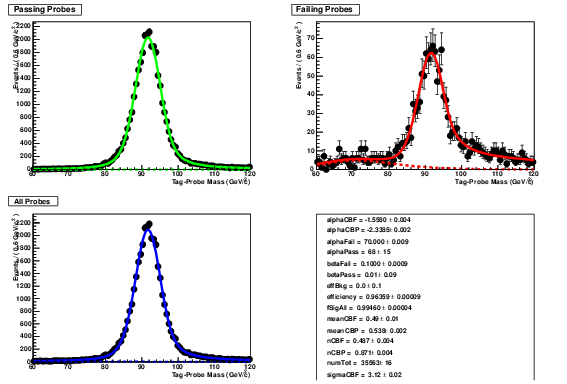
\includegraphics[width=0.8\textwidth]{Systematics/2012data_outputSCToGsfElectron.png}
\caption{Fitting of Supercluster to GSF Electrons for $\epsilon_{RECO}$ calculation.}
\label{fig:2012data_outputSCToGsfElectron}
\end{figure}
%2012data_outputSCToGsfElectron.eps





\begin{table}[htb]
\caption{%
    $\epsilon_{ID} \times \epsilon_{ISO}$ efficiency values from 2012 data and Monte Carlo simulations using the Tag and Probe method by fitting the signal and background.
}
\begin{center}
\begin{tabular}{ | c | c | c | c | c |}
      \hline
      $\eta$ coverage & $p_T$ range (GeV) & Efficiency (data) & Efficiency (MC) & Data/MC ratio \\ \hline \hline
     0.0 $<$ $\eta$ $<$ 0.8 & 10 $<$ $p_T$ $<$ 20 & 22.84\% $\pm$ 10.13\% & 54.53\% $\pm$ 13.17\% & 0.419 $\pm$ 0.212 \\ \hline
     0.8 $<$ $\eta$ $<$ 1.4 & 10 $<$ $p_T$ $<$ 20 & 37.14\% $\pm$ 0.54\% & 87.12\% $\pm$ 1.68\% & 0.426 $\pm$ 0.010 \\ \hline
     1.6 $<$ $\eta$ $<$ 2.0 & 10 $<$ $p_T$ $<$ 20 & 56.11\% $\pm$ 0.98\% & 93.84\% $\pm$ 4.98\% & 0.598 $\pm$ 0.033 \\ \hline
     2.0 $<$ $\eta$ $<$ 2.5 & 10 $<$ $p_T$ $<$ 20 & 56.39\% $\pm$ 1.43\% & 65.03\% $\pm$ 1.81\% & 0.867 $\pm$ 0.033 \\ \hline
     \hline
     0.0 $<$ $\eta$ $<$ 0.8 & 20 $<$ $p_T$ $<$ 40 & 96.15\% $\pm$ 0.44\% & 95.88\% $\pm$ 0.30\% & 1.003 $\pm$ 0.006 \\ \hline
     0.8 $<$ $\eta$ $<$ 1.4 & 20 $<$ $p_T$ $<$ 40 & 94.67\% $\pm$ 3.00\% & 96.75\% $\pm$ 1.88\% & 0.979 $\pm$ 0.036 \\ \hline
     1.6 $<$ $\eta$ $<$ 2.0 & 20 $<$ $p_T$ $<$ 40 & 95.31\% $\pm$ 0.79\% & 96.29\% $\pm$ 0.24\% & 0.990 $\pm$ 0.009 \\ \hline
     2.0 $<$ $\eta$ $<$ 2.5 & 20 $<$ $p_T$ $<$ 40 & 95.02\% $\pm$ 0.31\% & 92.90\% $\pm$ 3.64\% & 1.023 $\pm$ 0.040 \\ \hline
     \hline
     0.0 $<$ $\eta$ $<$ 0.8 & 40 $<$ $p_T$ $<$ 200 & 97.53\% $\pm$ 0.16\% & 98.22\% $\pm$ 0.05\% & 0.993 $\pm$ 0.002 \\ \hline
     0.8 $<$ $\eta$ $<$ 1.4 & 40 $<$ $p_T$ $<$ 200 & 98.08\% $\pm$ 0.07\% & 98.63\% $\pm$ 0.05\% & 0.994 $\pm$ 0.001 \\ \hline
     1.6 $<$ $\eta$ $<$ 2.0 & 40 $<$ $p_T$ $<$ 200 & 96.36\% $\pm$ 0.11\% & 97.47\% $\pm$ 1.31\% & 0.989 $\pm$ 0.013 \\ \hline
     2.0 $<$ $\eta$ $<$ 2.5 & 40 $<$ $p_T$ $<$ 200 & 95.61\% $\pm$ 0.30\% & 95.67\% $\pm$ 0.12\% & 0.999 $\pm$ 0.003 \\ \hline
    \end{tabular}
\end{center}
\label{tab:tagandprobe_ISO}
\end{table}


\begin{figure}[htb]
\centering
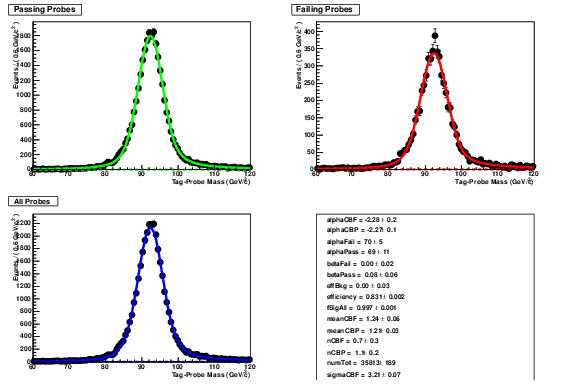
\includegraphics[width=0.8\textwidth]{Systematics/2012data_outputGsfElectronToId.png}
\caption{Fitting of GSF Electrons for to WP Medium for $\epsilon_{ISO}$ calculation.}
\label{fig:2012data_outputGsfElectronToId}
\end{figure}
%2012data_outputGsfElectronToId.eps



\begin{table}[htb]
\caption{%
    $\epsilon_{trigger}$ values for Ele8 Leg from 2012 data and Monte Carlo simulations using the Tag and Probe method by counting passing and failing probes.
}
\begin{center}

     \begin{tabular}{ | c | c | c | c | c |}
      \hline
      $\eta$ coverage & $p_T$ range (GeV) & Efficiency (data) & Efficiency (MC) & Data/MC ratio \\ \hline \hline
      0.0 $<$ $\eta$ $<$ 0.8 & 10 $<$ $p_T$ $<$ 20 & 96.03\% $\pm$ 0.37\% & 96.62\% $\pm$ 0.34\% & 0.994 $\pm$ 0.005 \\ \hline
      0.8 $<$ $\eta$ $<$ 1.4 & 10 $<$ $p_T$ $<$ 20 & 85.50\% $\pm$ 0.64\% & 88.63\% $\pm$ 0.56\% & 0.965 $\pm$ 0.009 \\ \hline
      1.6 $<$ $\eta$ $<$ 2.0 & 10 $<$ $p_T$ $<$ 20 & 84.15\% $\pm$ 0.99\% & 83.76\% $\pm$ 1.02\% & 1.005 $\pm$ 0.017 \\ \hline
      2.0 $<$ $\eta$ $<$ 2.5 & 10 $<$ $p_T$ $<$ 20 & 84.80\% $\pm$ 1.04\% & 88.53\% $\pm$ 0.98\% & 0.958 $\pm$ 0.016 \\ \hline
      \hline
      0.0 $<$ $\eta$ $<$ 0.8 & 20 $<$ $p_T$ $<$ 40 & 98.19\% $\pm$ 0.05\% & 98.42\% $\pm$ 0.04\% & 0.998 $\pm$ 0.001 \\ \hline
      0.8 $<$ $\eta$ $<$ 1.4 & 20 $<$ $p_T$ $<$ 40 & 92.99\% $\pm$ 0.11\% & 94.14\% $\pm$ 0.10\% & 0.988 $\pm$ 0.002 \\ \hline
      1.6 $<$ $\eta$ $<$ 2.0 & 20 $<$ $p_T$ $<$ 40 & 89.07\% $\pm$ 0.20\% & 89.47\% $\pm$ 0.20\% & 0.996 $\pm$ 0.003 \\ \hline
      2.0 $<$ $\eta$ $<$ 2.5 & 20 $<$ $p_T$ $<$ 40 & 92.59\% $\pm$ 0.19\% & 92.53\% $\pm$ 0.20\% & 1.001 $\pm$ 0.003 \\ \hline
      \hline
      0.0 $<$ $\eta$ $<$ 0.8 & 40 $<$ $p_T$ $<$ 200 & 98.81\% $\pm$ 0.04\% & 99.11\% $\pm$ 0.03\% & 0.997 $\pm$ 0.001 \\ \hline
      0.8 $<$ $\eta$ $<$ 1.4 & 40 $<$ $p_T$ $<$ 200 & 96.92\% $\pm$ 0.07\% & 97.42\% $\pm$ 0.06\% & 0.995 $\pm$ 0.001 \\ \hline
      1.6 $<$ $\eta$ $<$ 2.0 & 40 $<$ $p_T$ $<$ 200 & 93.22\% $\pm$ 0.15\% & 93.73\% $\pm$ 0.13\% & 0.995 $\pm$ 0.002 \\ \hline
      2.0 $<$ $\eta$ $<$ 2.5 & 40 $<$ $p_T$ $<$ 200 & 94.74\% $\pm$ 0.15\% & 95.04\% $\pm$ 0.14\% & 0.997 $\pm$ 0.002 \\ \hline
      \end{tabular}
\end{center}
\label{tab:tagandprobe_8}
\end{table}

\begin{table}[htb]
\caption{%
    $\epsilon_{trigger}$ values for Ele17 Leg from 2012 data and Monte Carlo simulations using the Tag and Probe method by counting passing and failing probes.
}
\begin{center}

    \begin{tabular}{ | c | c | c | c | c |}
      \hline
      $\eta$ coverage & $p_T$ range (GeV) & Efficiency (data) & Efficiency (MC) & Data/MC ratio \\ \hline \hline
      0.0 $<$ $\eta$ $<$ 0.8 & 10 $<$ $p_T$ $<$ 20 & 48.80\% $\pm$ 0.92\% & 57.97\% $\pm$ 0.91\% & 0.842 $\pm$ 0.021 \\ \hline
      0.8 $<$ $\eta$ $<$ 1.4 & 10 $<$ $p_T$ $<$ 20 & 33.01\% $\pm$ 0.85\% & 46.75\% $\pm$ 0.87\% & 0.706 $\pm$ 0.022 \\ \hline
      1.6 $<$ $\eta$ $<$ 2.0 & 10 $<$ $p_T$ $<$ 20 & 47.63\% $\pm$ 1.34\% & 47.23\% $\pm$ 1.37\% & 1.008 $\pm$ 0.041 \\ \hline
      2.0 $<$ $\eta$ $<$ 2.5 & 10 $<$ $p_T$ $<$ 20 & 40.66\% $\pm$ 1.41\% & 50.52\% $\pm$ 1.52\% & 0.805 $\pm$ 0.037 \\ \hline
      \hline
      0.0 $<$ $\eta$ $<$ 0.8 & 20 $<$ $p_T$ $<$ 40 & 98.49\% $\pm$ 0.04\% & 98.86\% $\pm$ 0.04\% & 0.996 $\pm$ 0.001 \\ \hline
      0.8 $<$ $\eta$ $<$ 1.4 & 20 $<$ $p_T$ $<$ 40 & 93.45\% $\pm$ 0.11\% & 94.62\% $\pm$ 0.10\% & 0.988 $\pm$ 0.002 \\ \hline
      1.6 $<$ $\eta$ $<$ 2.0 & 20 $<$ $p_T$ $<$ 40 & 89.71\% $\pm$ 0.19\% & 89.98\% $\pm$ 0.19\% & 0.997 $\pm$ 0.003 \\ \hline
      2.0 $<$ $\eta$ $<$ 2.5 & 20 $<$ $p_T$ $<$ 40 & 93.67\% $\pm$ 0.18\% & 93.59\% $\pm$ 0.18\% & 1.001 $\pm$ 0.003 \\ \hline
      \hline
      0.0 $<$ $\eta$ $<$ 0.8 & 40 $<$ $p_T$ $<$ 200 & 99.05\% $\pm$ 0.03\% & 99.41\% $\pm$ 0.03\% & 0.996 $\pm$ 0.000 \\ \hline
      0.8 $<$ $\eta$ $<$ 1.4 & 40 $<$ $p_T$ $<$ 200 & 97.41\% $\pm$ 0.07\% & 97.92\% $\pm$ 0.06\% & 0.995 $\pm$ 0.001 \\ \hline
      1.6 $<$ $\eta$ $<$ 2.0 & 40 $<$ $p_T$ $<$ 200 & 93.90\% $\pm$ 0.14\% & 94.38\% $\pm$ 0.13\% & 0.995 $\pm$ 0.002 \\ \hline
      2.0 $<$ $\eta$ $<$ 2.5 & 40 $<$ $p_T$ $<$ 200 & 95.93\% $\pm$ 0.13\% & 96.17\% $\pm$ 0.12\% & 0.998 $\pm$ 0.002 \\ \hline
    \end{tabular}
\end{center}
\label{tab:tagandprobe_17}
\end{table}



\section{Background shape systematic uncertainties}



\subsection{Upper and Lower Side Band Comparison}

In order to estimate how MC repoduced the shape in data for the sideband we plot both data-MC and the ratio $\dfrac{data}{MC}$.  In particular we also compare
the shapes in the lower and upper sidebands to get a more acurate picture of the shape.  This give a more accurate representation of the error in the
background that looking at the shape difference between $m_{jjll} p_{T}$-reweighted and $m_{jjll}$ non $p_{T}$-weighted. The exclusive $\PZ$+Jets samples (1-4 jets)
are $m_{jjll} p_{T}$-weighted.  The data and MC are normalized to unity before comparisons. The plots for are three categories are
shown in Figures ~\ref{fig:0tag_sideband_up_down}, ~\ref{fig:1tag_sideband_up_down}, and ~\ref{fig:2tag_sideband_up_down}.  

%%%%%%%%%
\begin{figure}[htb!]
%\begin{center}
\centerline{
%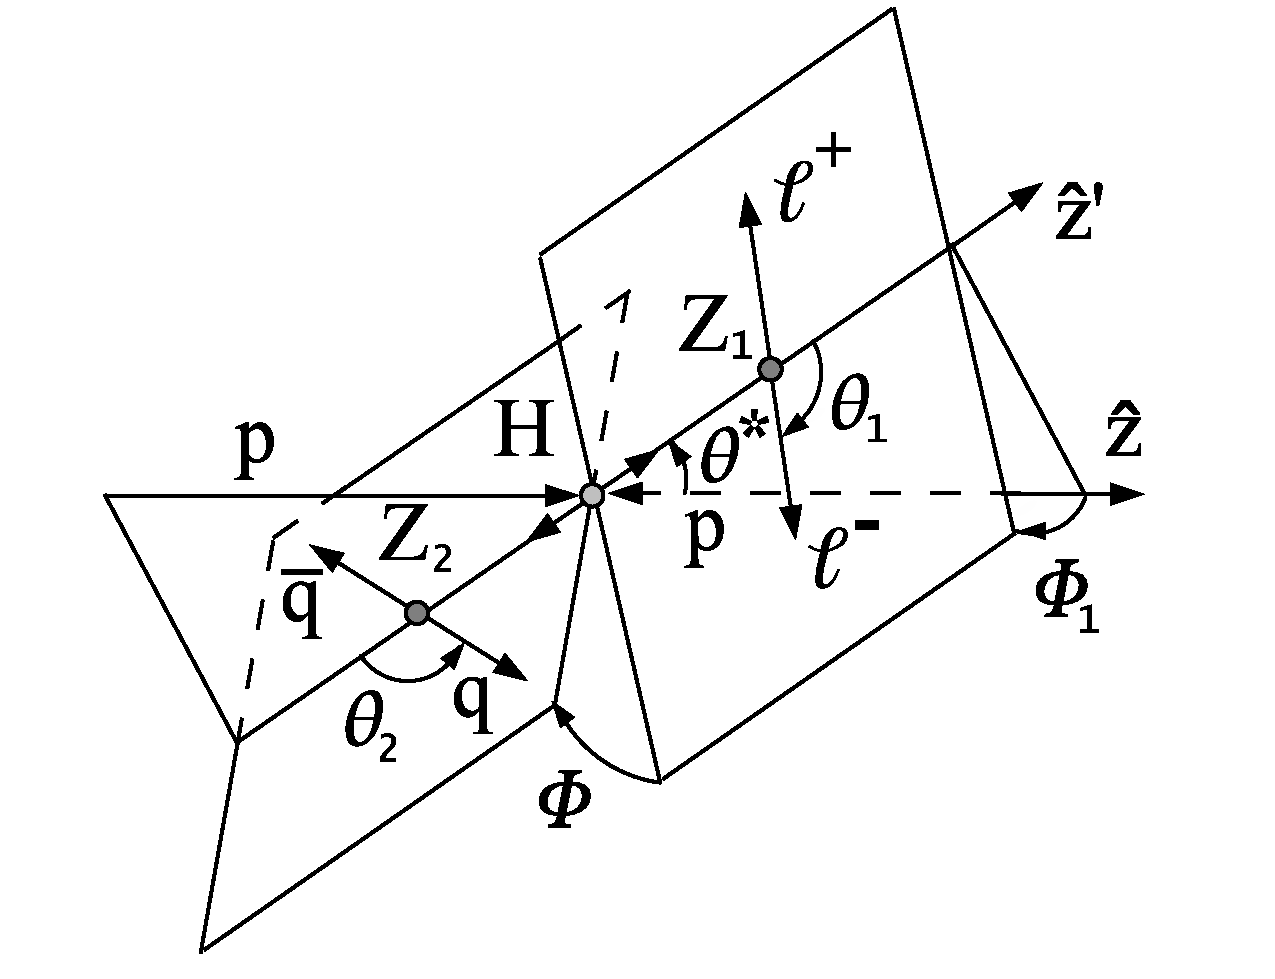
\includegraphics[height=2.5in]{plots/angles-HZZ2l2q}
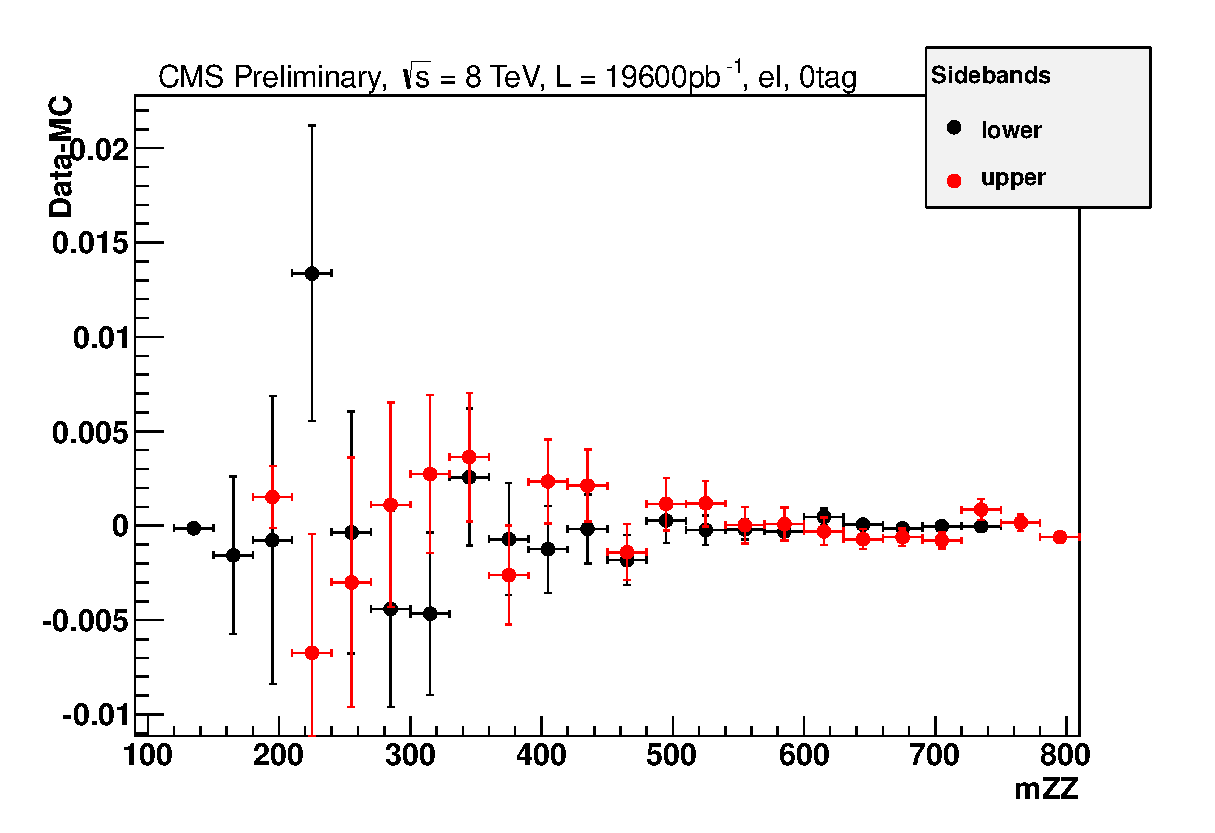
\includegraphics[height=2.5in]{Systematics/plots/subtract_el_2_0}
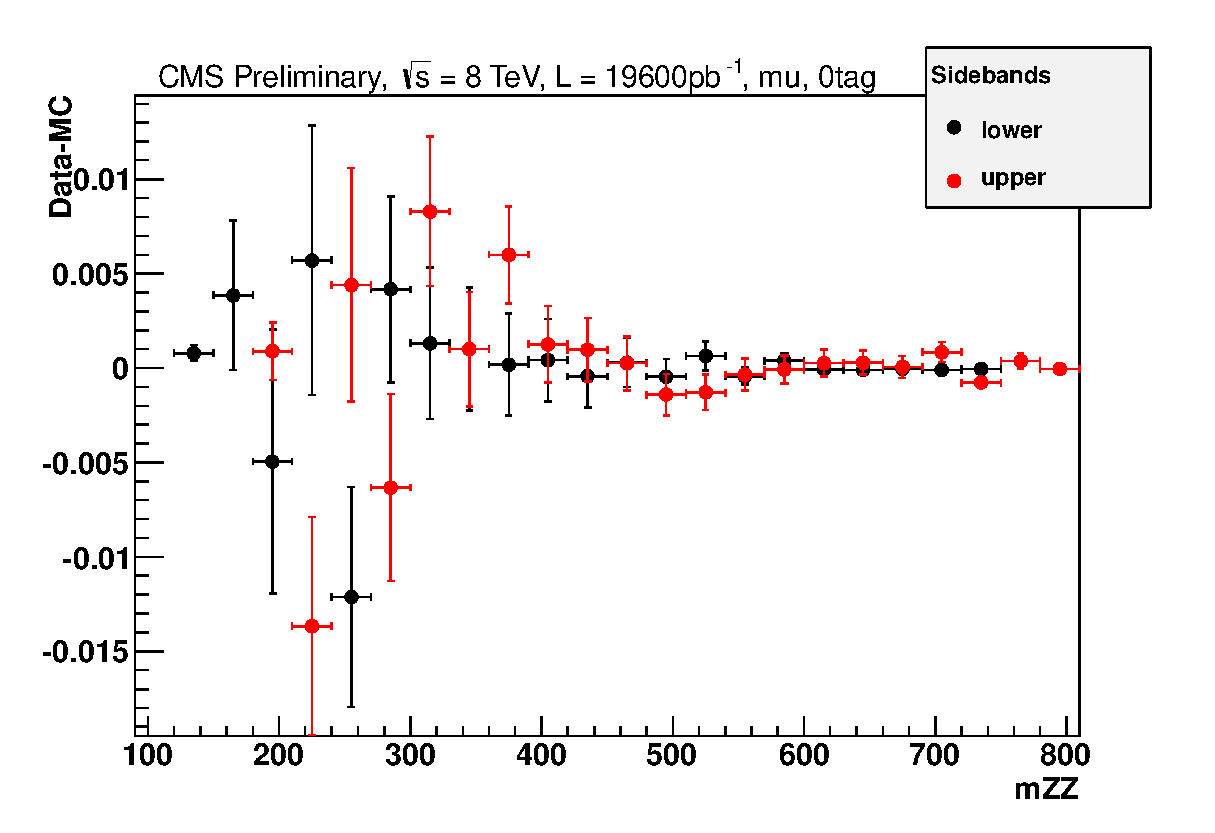
\includegraphics[height=2.5in]{Systematics/plots/subtract_mu_2_0}}
\centerline{
\\
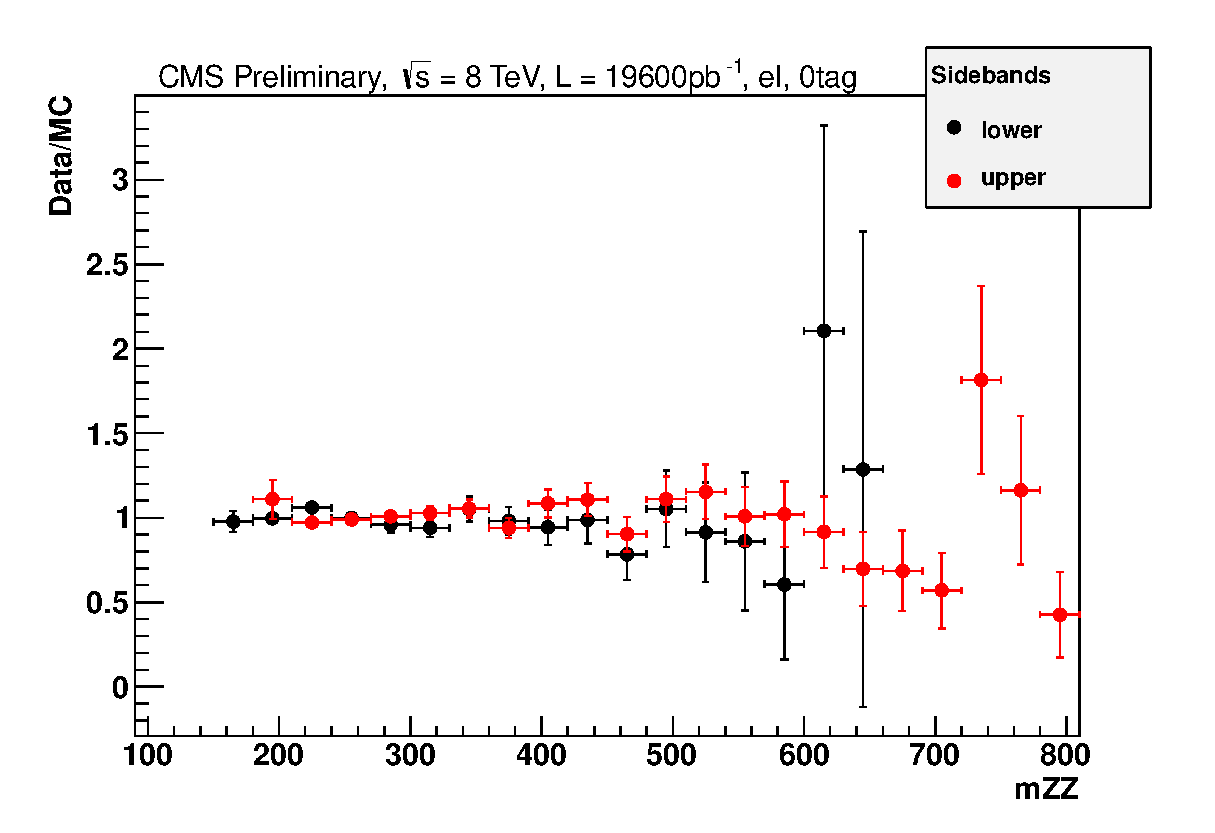
\includegraphics[height=2.5in]{Systematics/plots/divide_el_2_0}
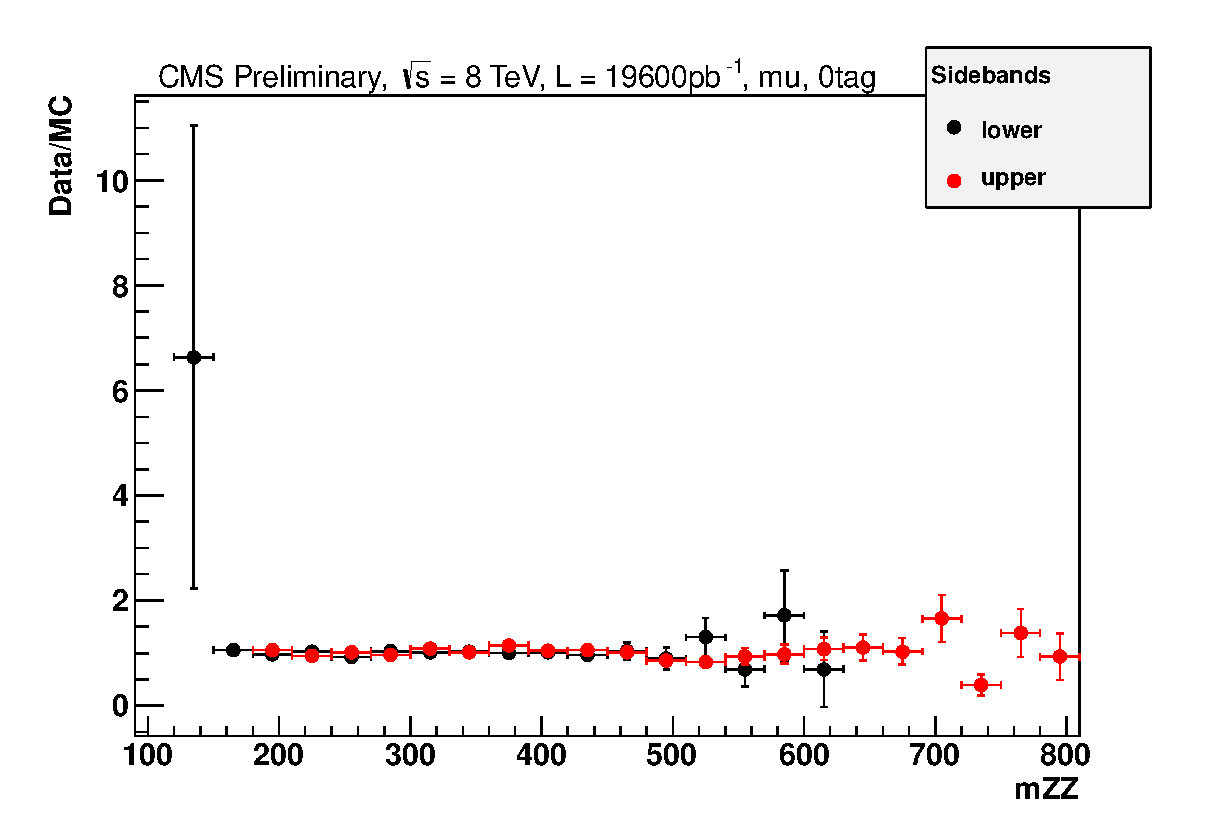
\includegraphics[height=2.5in]{Systematics/plots/divide_mu_2_0}
\\
%\includegraphics[height=2.5in]{plots/angles-Graviton-all2}
}
%\end{center}
\caption{Comparing Data and MC in the 0 BTag regions for both the upper sideband and lower sideband regions. Data and MC are first normalized to unity before the comparisons. All plots are looking as a function of the mass of the two Zs. Top left: Data - MC for electrons.  Top right: Data - MC for muons.  Bottom left: Data/MC for electrons.  Bottom right: Data/MC for muons.
\label{fig:0tag_sideband_up_down}}  
\end{figure}
%%%%%%%%%
\begin{figure}[htb!]
%\begin{center}
\centerline{
%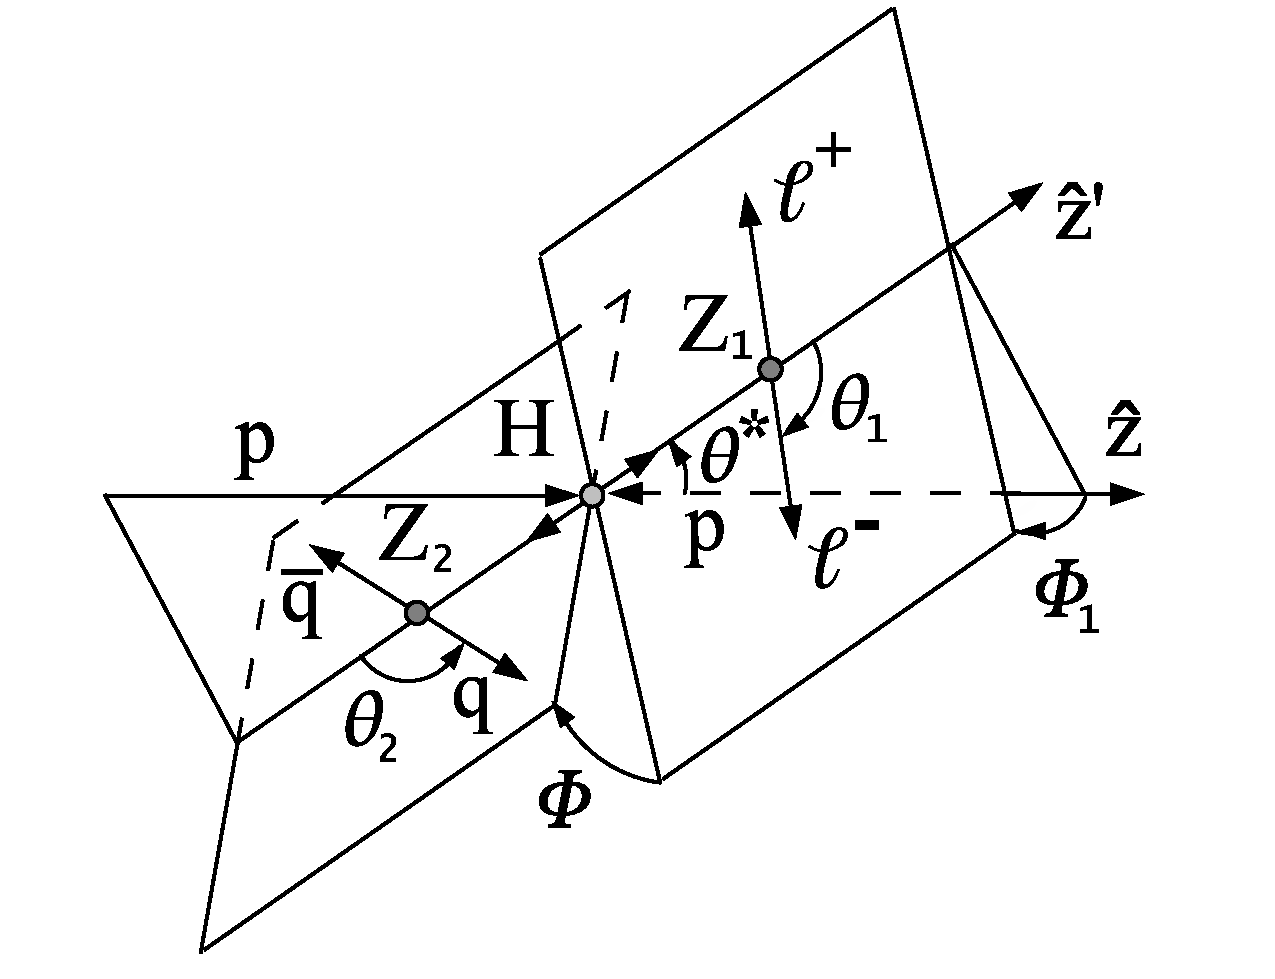
\includegraphics[height=2.5in]{plots/angles-HZZ2l2q}
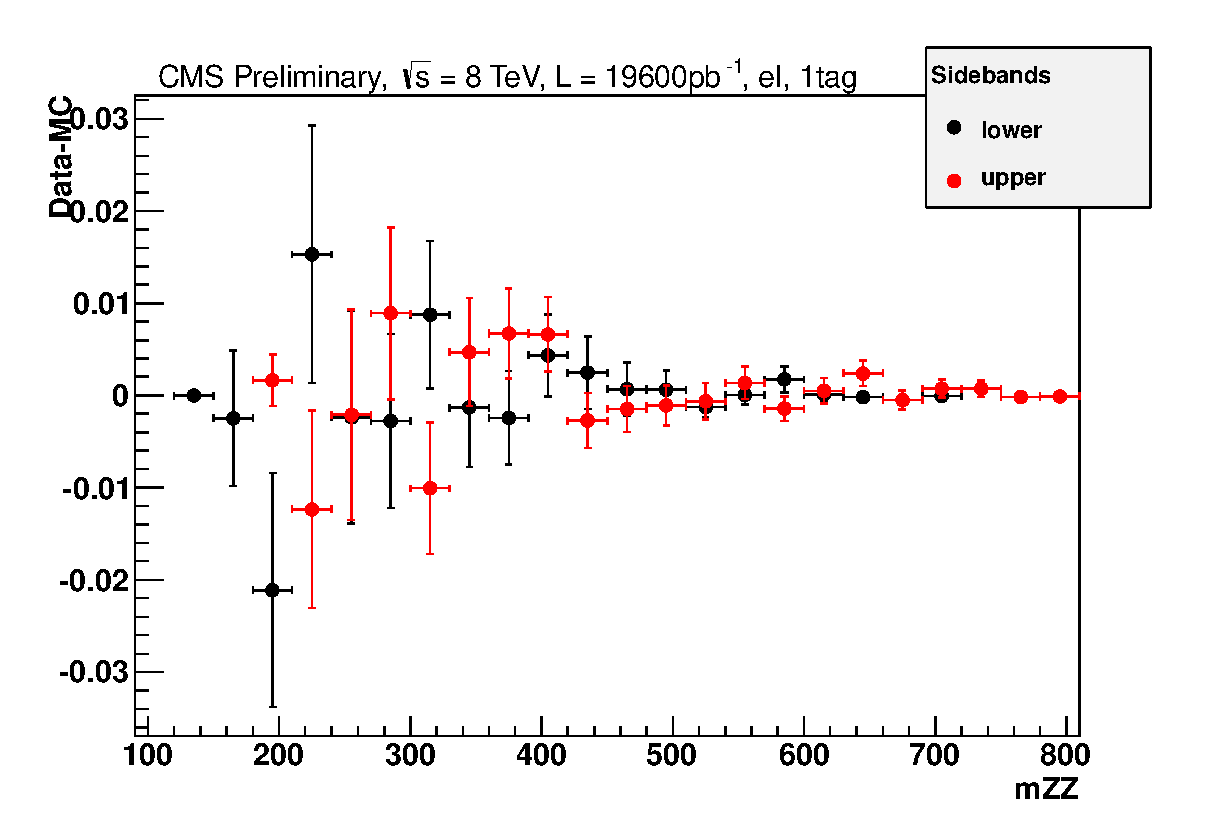
\includegraphics[height=2.5in]{Systematics/plots/subtract_el_2_1}
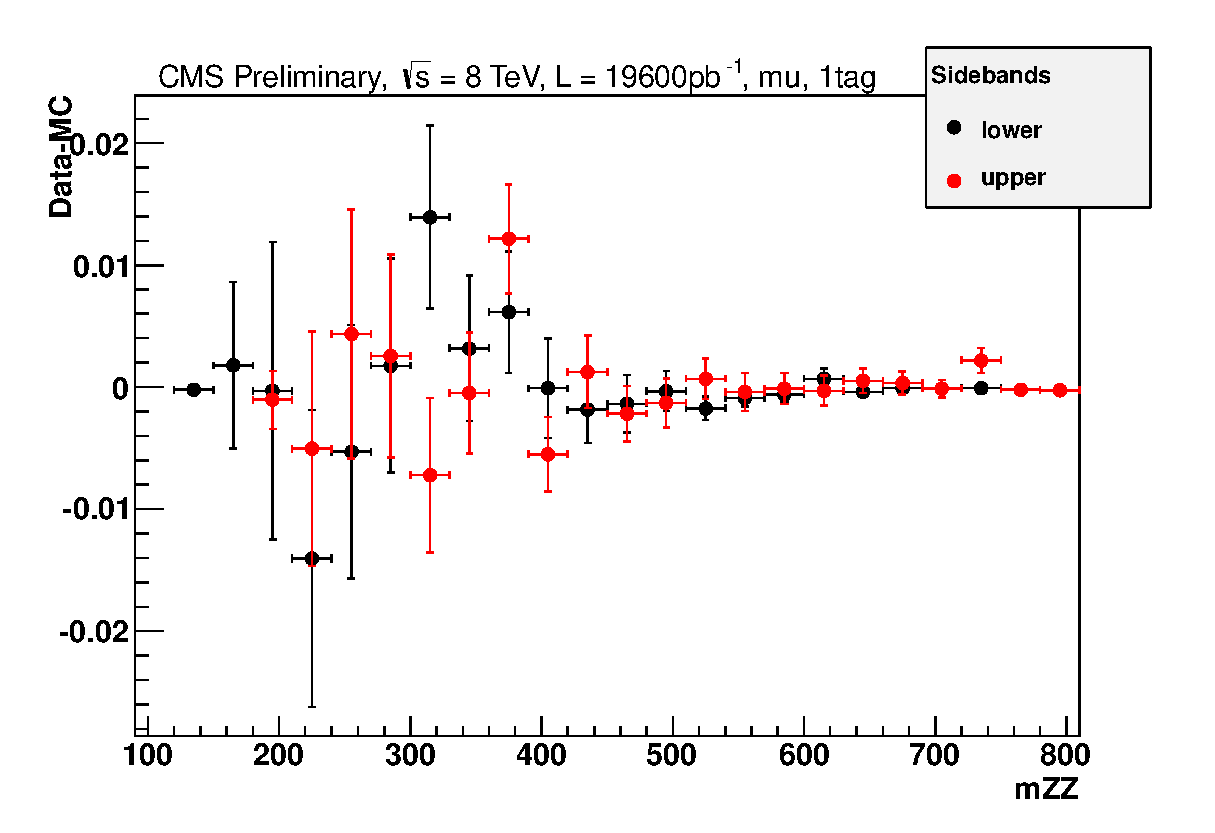
\includegraphics[height=2.5in]{Systematics/plots/subtract_mu_2_1}}
\centerline{
\\
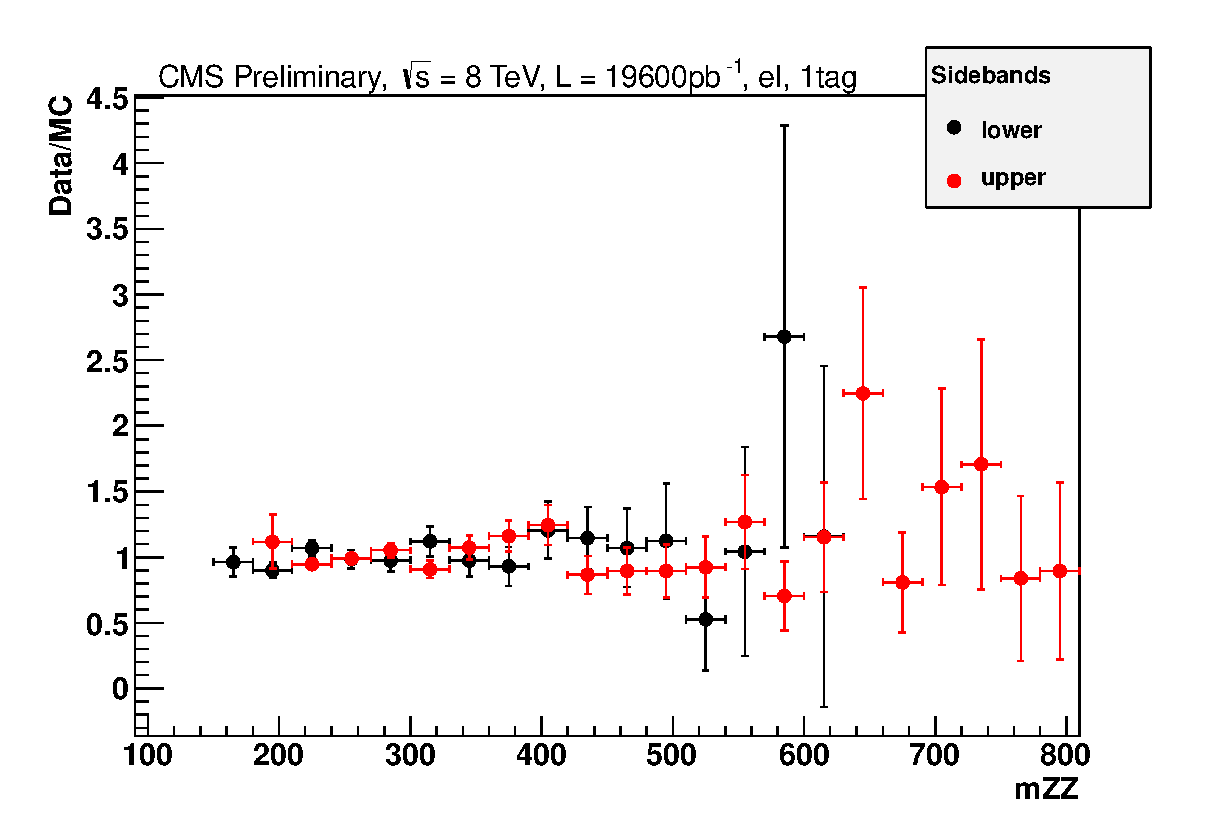
\includegraphics[height=2.5in]{Systematics/plots/divide_el_2_1}
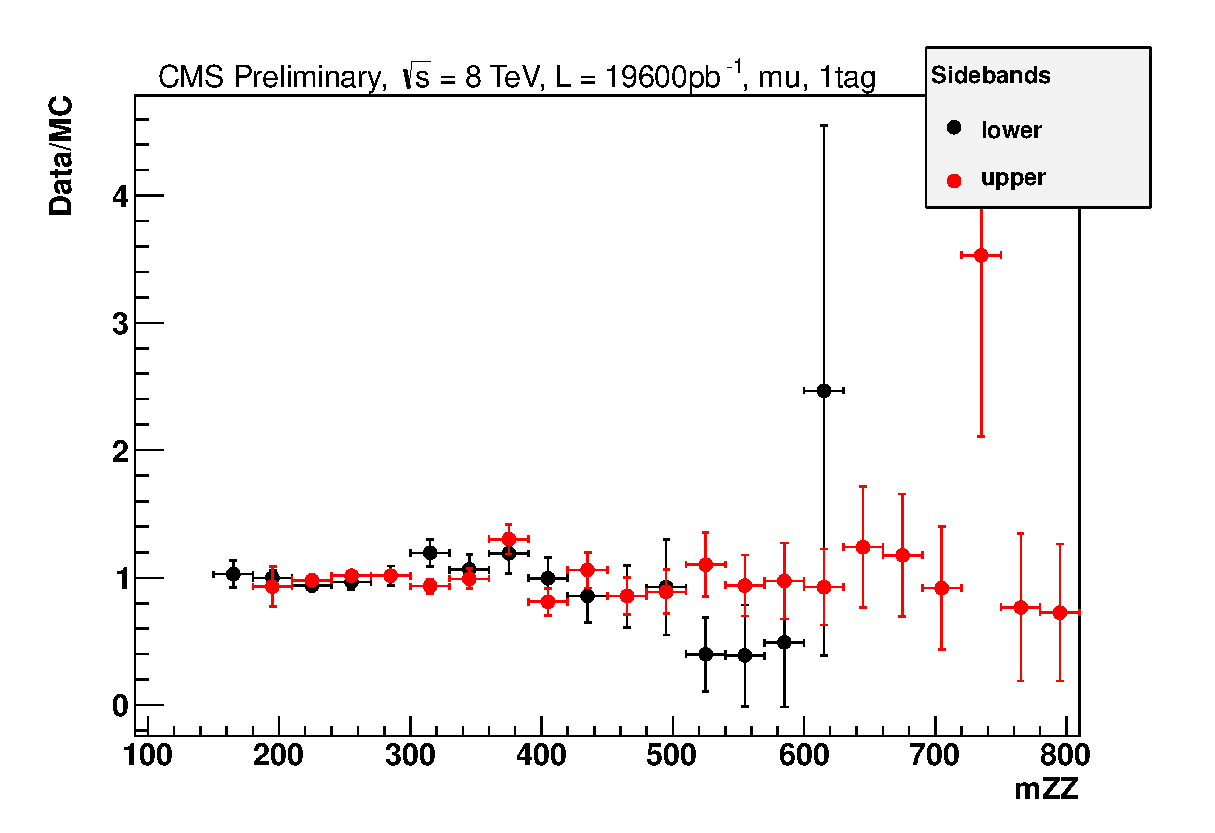
\includegraphics[height=2.5in]{Systematics/plots/divide_mu_2_1}
\\
%\includegraphics[height=2.5in]{plots/angles-Graviton-all2}
}
%\end{center}
\caption{Comparing Data and MC in the 1 BTag regions for both the upper sideband and lower sideband regions. Data and MC are first normalized to unity before the comparisons. All plots are looking as a function of the mass of the two Zs. Top left: Data - MC for electrons.  Top right: Data - MC for muons.  Bottom left: Data/MC for electrons.  Bottom right: Data/MC for muons.
\label{fig:1tag_sideband_up_down}}  
\end{figure}
%%%%%%%%%
\begin{figure}[htb!]
%\begin{center}
\centerline{
%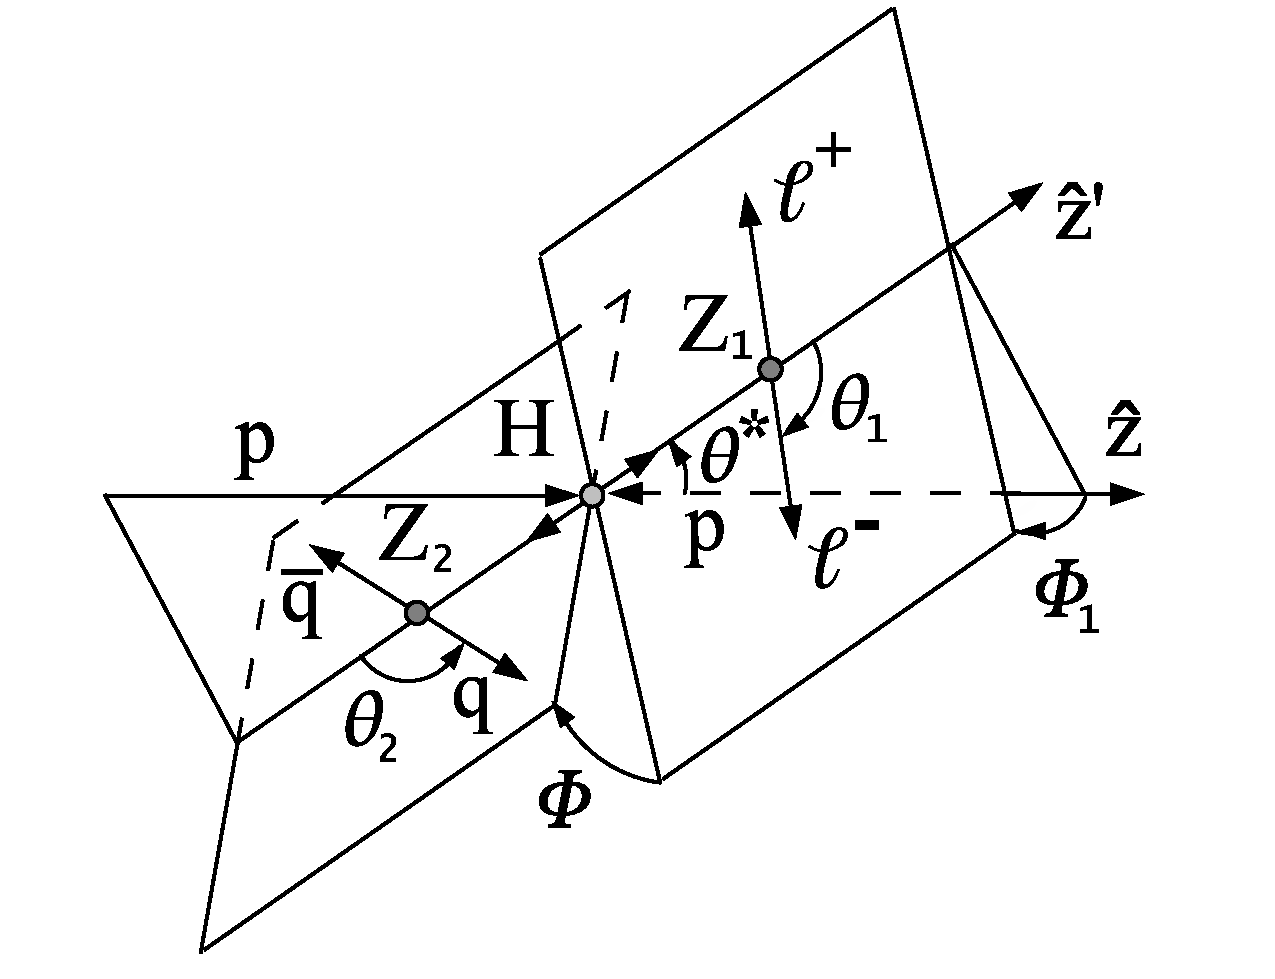
\includegraphics[height=2.5in]{plots/angles-HZZ2l2q}
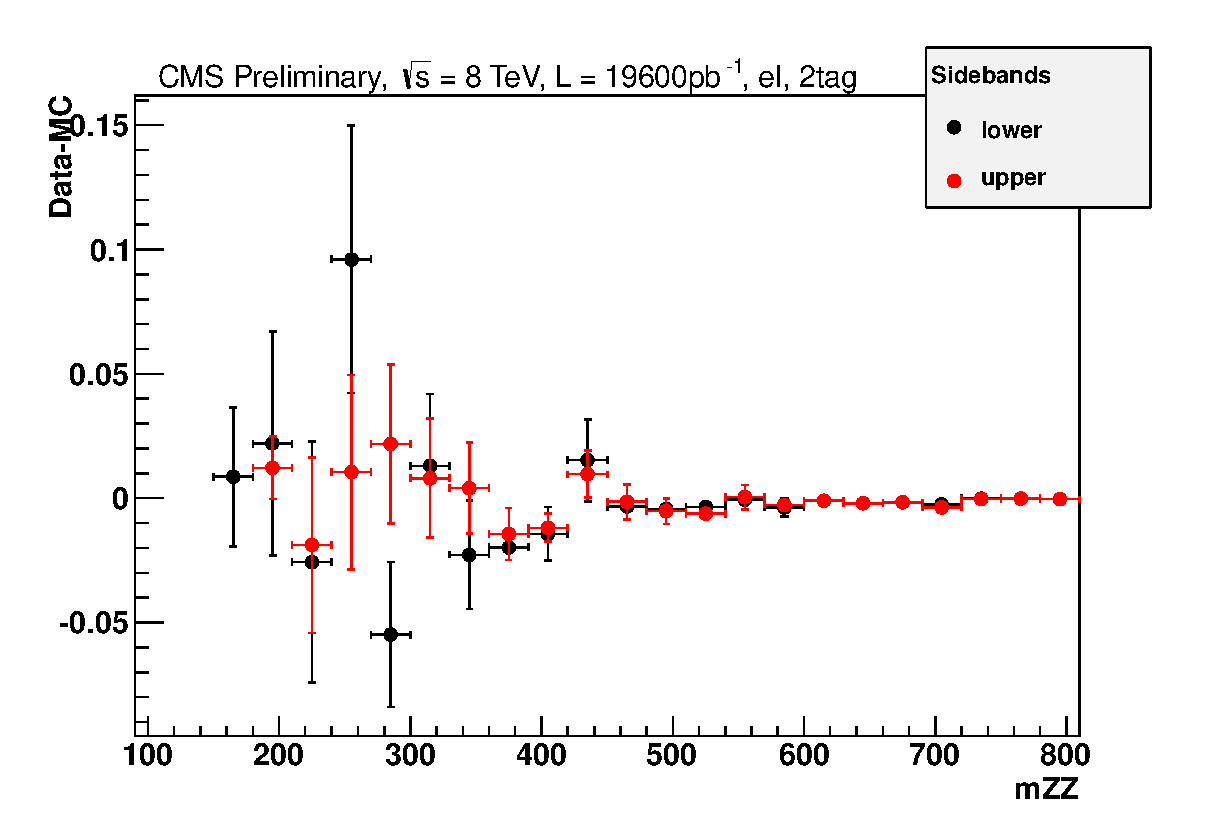
\includegraphics[height=2.5in]{Systematics/plots/subtract_el_2_2}
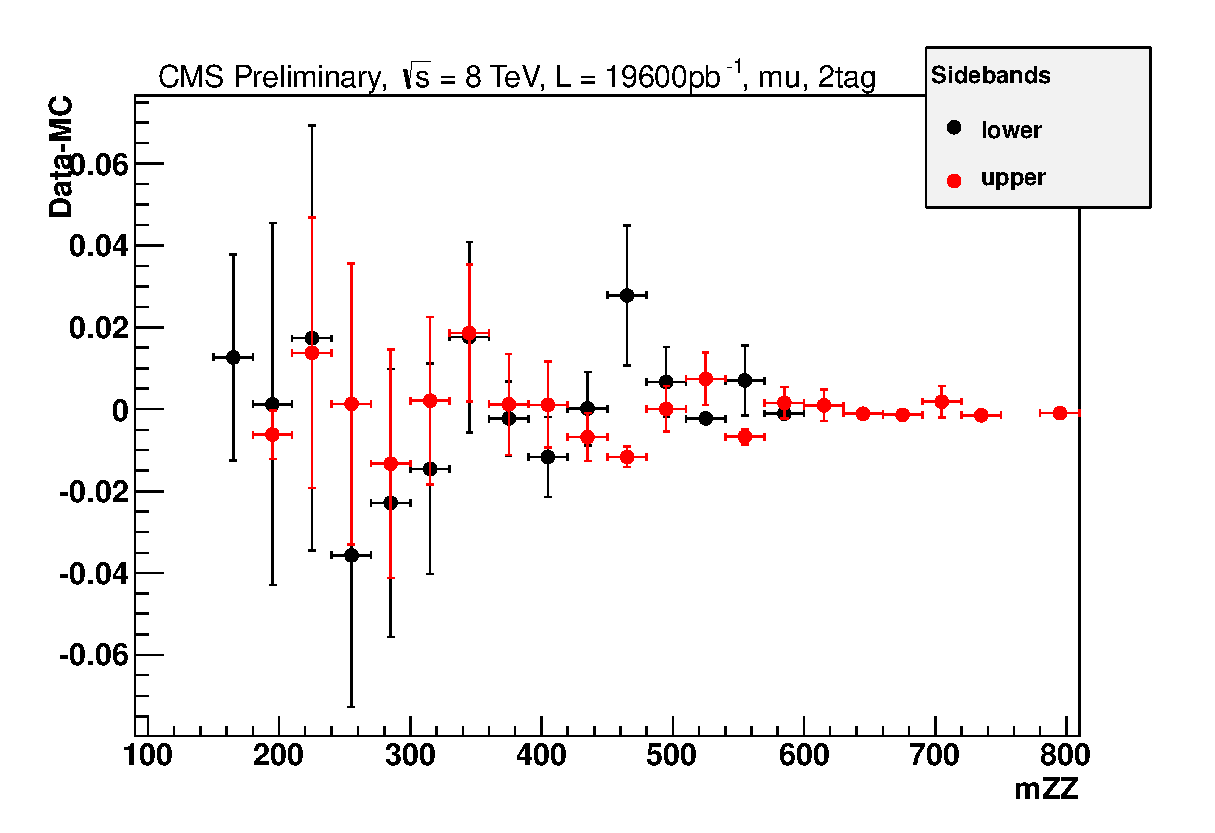
\includegraphics[height=2.5in]{Systematics/plots/subtract_mu_2_2}}
\centerline{
\\
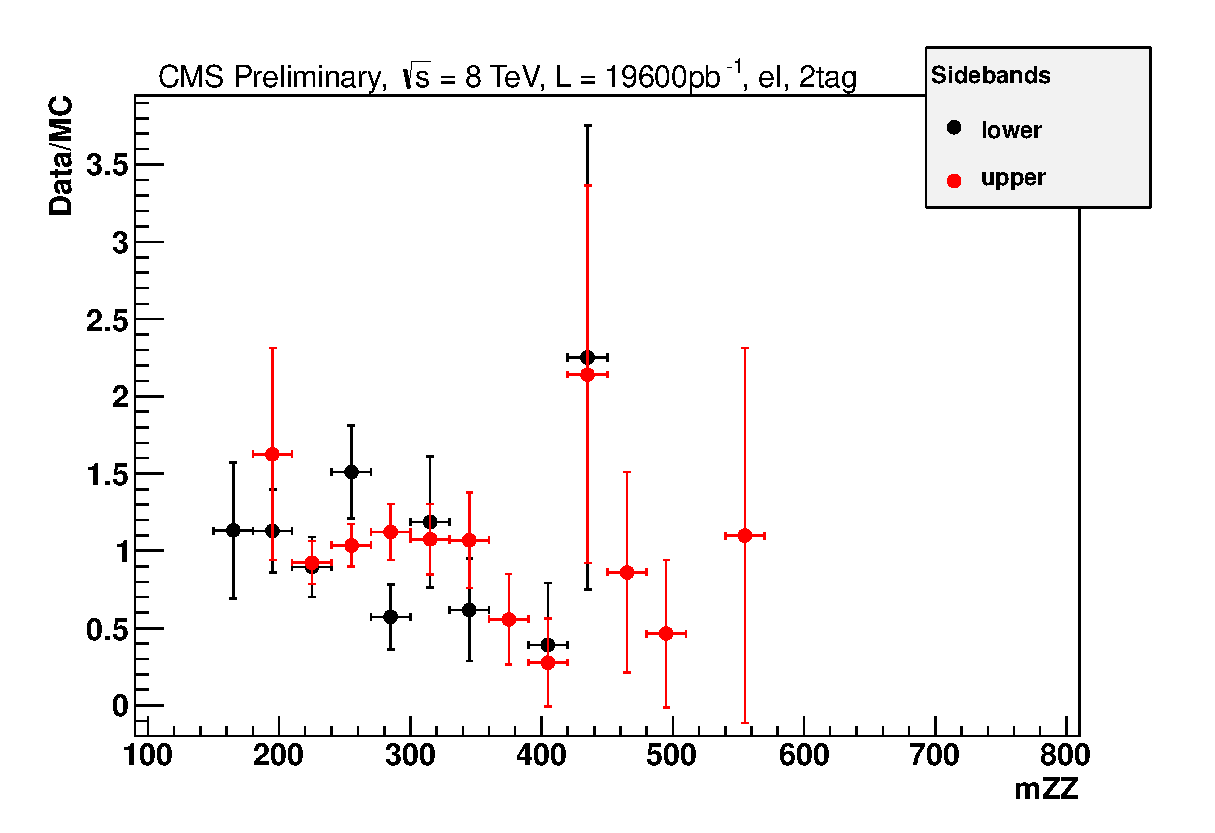
\includegraphics[height=2.5in]{Systematics/plots/divide_el_2_2}
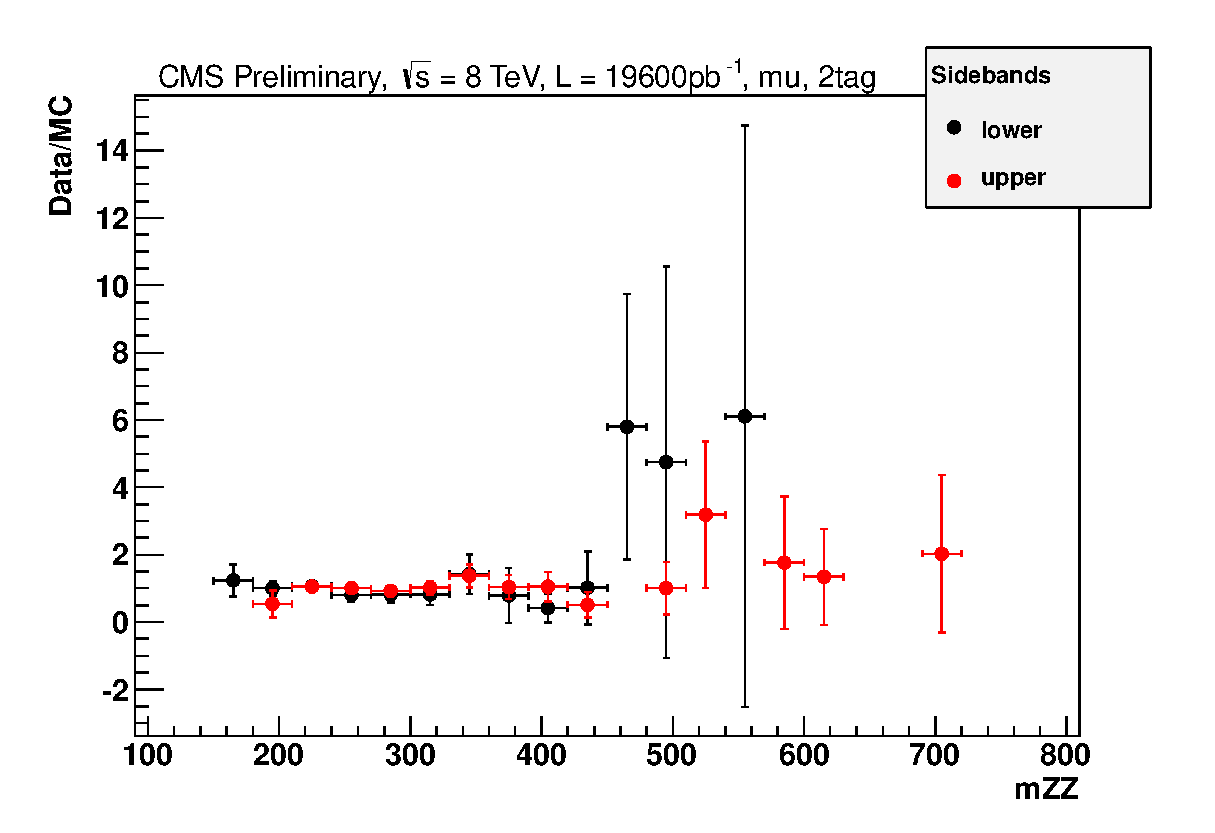
\includegraphics[height=2.5in]{Systematics/plots/divide_mu_2_2}
\\
%\includegraphics[height=2.5in]{plots/angles-Graviton-all2}
}
%\end{center}
\caption{Comparing Data and MC in the 2 BTag regions for both the upper sideband and lower sideband regions. Data and MC are first normalized to unity before the comparisons. All plots are looking as a function of the mass of the two Zs. Top left: Data - MC for electrons.  Top right: Data - MC for muons.  Bottom left: Data/MC for electrons.  Bottom right: Data/MC for muons.
\label{fig:2tag_sideband_up_down}}  
\end{figure}
%%%%%%%%%




%\subsection{Subsection heading}

%\subsubsection{Subsubsection heading}

